\documentclass[border=6pt]{standalone}
\usepackage{tikz}
% ---- real Helvetica-clone sans-serif (text + math), matching Figures 2 and 7 ----
\usepackage{tgheros}\renewcommand{\familydefault}{\sfdefault}
\usepackage[T1]{fontenc}
\usepackage{sansmath}
\usetikzlibrary{positioning,calc,arrows.meta,shapes.geometric}
% ---- shared palette: pale fills + matching mid-tone borders, black text ----
% R2-11a: figure recoloured to greyscale (reviewer: colours in Figure 1 are unnecessary).
% Node types are now distinguished by fill shade and border only, all monochrome.
\definecolor{txt}{HTML}{000000}
\definecolor{gyF}{HTML}{F2F2F2}\definecolor{gyB}{HTML}{000000}   % light grey fill (input / decision / negative)
\definecolor{blF}{HTML}{FFFFFF}\definecolor{blB}{HTML}{000000}   % white fill (off-device compute)
\definecolor{gnF}{HTML}{E8E8E8}\definecolor{gnB}{HTML}{000000}   % grey fill (on-device measurement)
\definecolor{rdF}{HTML}{C8C8C8}\definecolor{rdB}{HTML}{000000}   % darker grey fill (headline result)
\definecolor{socB}{HTML}{000000}
\begin{document}\sansmath
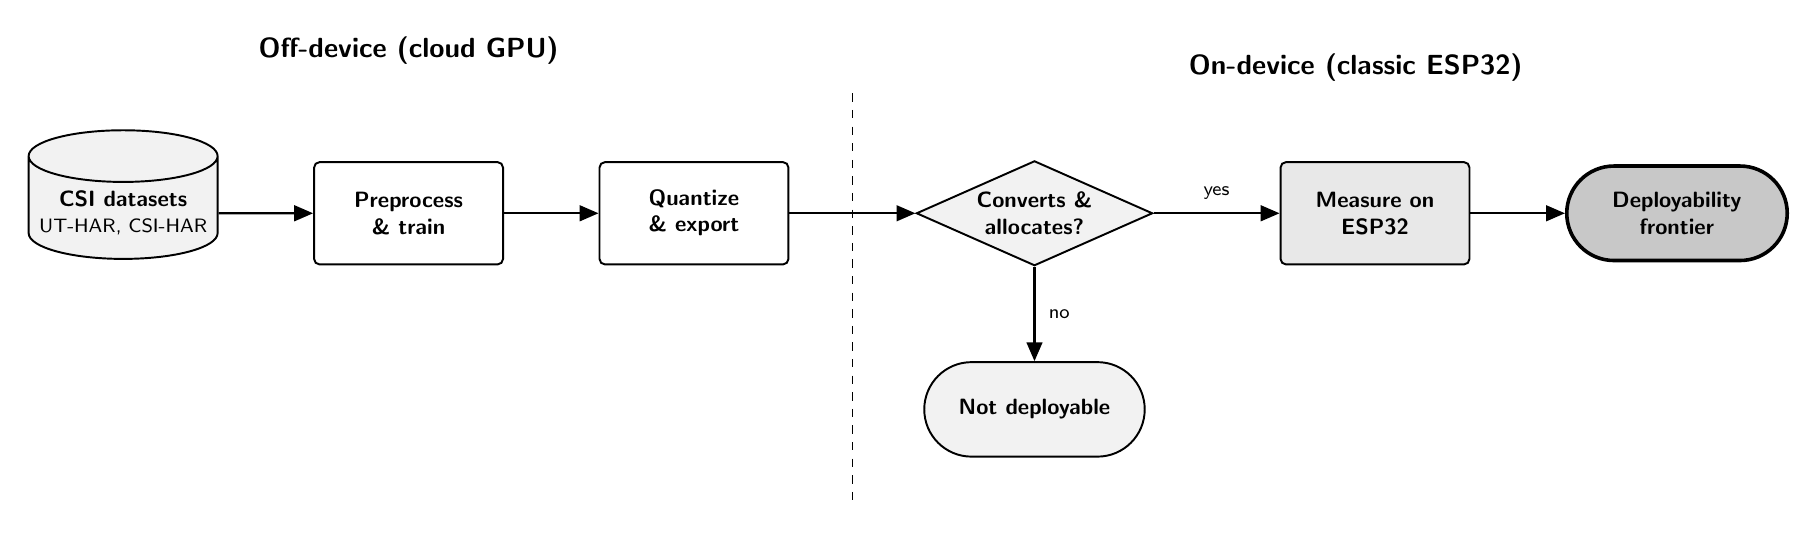
\begin{tikzpicture}[
  font=\footnotesize,text=txt,node distance=12mm,
  >={Triangle[length=2.4mm,width=2mm]},
  every edge/.style={draw,line width=0.8pt,-{Triangle[length=2.4mm,width=2mm]}},
  proc/.style={rounded corners=2pt,line width=0.7pt,fill=blF,draw=blB,align=center,inner sep=3pt,minimum width=24mm,minimum height=13mm},
  meas/.style={proc,fill=gnF,draw=gnB},
  data/.style={cylinder,shape border rotate=90,aspect=0.28,line width=0.7pt,fill=gyF,draw=gyB,align=center,inner sep=3pt,minimum width=24mm,minimum height=16mm},
  dec/.style={diamond,aspect=2.1,line width=0.7pt,fill=gyF,draw=gyB,align=center,inner sep=1pt,minimum width=30mm},
  term/.style={rounded corners=6mm,line width=0.7pt,align=center,inner sep=3pt,minimum width=28mm,minimum height=12mm},
  good/.style={term,fill=rdF,draw=rdB,line width=1.3pt},
  bad/.style={term,fill=gyF,draw=gyB},
  ]

% ---- main chain ----
\node[data] (ds) {\textbf{CSI datasets}\\\scriptsize UT-HAR, CSI-HAR};
\node[proc,right=of ds] (pp) {\textbf{Preprocess}\\\textbf{\& train}};
\node[proc,right=of pp] (qz) {\textbf{Quantize}\\\textbf{\& export}};
\node[dec,right=16mm of qz] (dc) {\textbf{Converts \&}\\\textbf{allocates?}};
\node[meas,right=16mm of dc] (ms) {\textbf{Measure on}\\\textbf{ESP32}};
\node[good,right=of ms] (fr) {\textbf{Deployability}\\\textbf{frontier}};
\node[bad,below=12mm of dc] (nd) {\textbf{Not deployable}};

% ---- edges ----
\draw (ds) edge (pp);
\draw (pp) edge (qz);
\draw (qz) edge (dc);
\draw (dc) edge node[above=0.5mm,font=\scriptsize]{yes} (ms);
\draw (dc) edge node[right=0.5mm,font=\scriptsize]{no} (nd);
\draw (ms) edge (fr);

% ---- zone divider + section labels ----
\coordinate (mid) at ($(qz.east)!0.5!(dc.west)$);
\draw[gyB,line width=0.6pt,dashed] ([yshift=9mm]mid|-fr.north) -- ([yshift=-6mm]mid|-nd.south);
\node[font=\bfseries,text=socB,anchor=south] at ($(ds.north)!0.5!(qz.north)+(0,9mm)$) {Off-device (cloud GPU)};
\node[font=\bfseries,text=socB,anchor=south] at ($(dc.north)!0.5!(fr.north)+(0,9mm)$) {On-device (classic ESP32)};

\end{tikzpicture}
\end{document}
